
\documentclass{article}
\usepackage{smc}
\usepackage{times}
\usepackage{ifpdf}
\bibliographystyle{plainnat}
\usepackage[english]{babel}
\usepackage[numbers]{natbib}

%user defined variables
\def\papertitle{A new way to Conditioned Play Audiometry: Exploring  gamification opportunities}
\def\firstauthor{Emil Sønderskov Hansen}
\def\thirdauthor{Stefania Serafin}

\newif\ifpdf
\ifx\pdfoutput\relax
\else
   \ifcase\pdfoutput
      \pdffalse
   \else
      \pdftrue
\fi

\ifpdf % compiling with pdflatex
  \usepackage[pdftex,
    pdftitle={\papertitle},
    pdfauthor={\firstauthor, \secondauthor, \thirdauthor},
    bookmarksnumbered, % use section numbers with bookmarks
    pdfstartview=XYZ % start with zoom=100% instead of full screen; 
                     % especially useful if working with a big screen :-)
   ]{hyperref}
  %\pdfcompresslevel=9

  \usepackage[pdftex]{graphicx}
  % declare the path(s) where your graphic files are and their extensions so 
  %you won't have to specify these with every instance of \includegraphics
  \graphicspath{{./figures/}}
  \DeclareGraphicsExtensions{.pdf,.jpeg,.png}

  \usepackage[figure,table]{hypcap}

\else % compiling with latex
  \usepackage[dvips,
    bookmarksnumbered, % use section numbers with bookmarks
    pdfstartview=XYZ % start with zoom=100% instead of full screen
  ]{hyperref}  % hyperrefs are active in the pdf file after conversion

  \usepackage[dvips]{epsfig,graphicx}
  % declare the path(s) where your graphic files are and their extensions so 
  %you won't have to specify these with every instance of \includegraphics
  \graphicspath{{./figures/}}
  \DeclareGraphicsExtensions{.eps}

  \usepackage[figure,table]{hypcap}
\fi

\hypersetup{
    colorlinks,%
    citecolor=black,%
    filecolor=black,%
    linkcolor=black,%
    urlcolor=black
}

\title{\papertitle}

 \threeauthors
   {\firstauthor} {Aalborg University CPH \\ %
     {\tt \href{mailto:esha19@student.aau.dk}{esha19@student.aau.dk}}}
   {\secondauthor} {Aalborg University CPH \\ %
     {\tt \href{mailto:smkk19@student.aau.dk}{smkk19@student.aau.dk}}}
   {\thirdauthor} {Multisensory Experience Lab \\ %
   {\tt \href{mailto:adj@create.aau.dk}{adj@create.aau.dk}}
     {\tt \href{mailto:sts@create.aau.dk}{sts@create.aau.dk}}}
     
 \author{
  Emil Sønderskov Hansen \\ Aalborg University CPH \\
  \texttt{\href{mailto:esha19@student.aau.dk}{esha19@student.aau.dk}}
  \and
  Stefania Serafin \\ Multisensory Experience Lab \\
  \texttt{\href{mailto:sts@create.aau.dk}{sts@create.aau.dk}}
}
     
     



% ***************************************** the document starts here ***************
\begin{document}

\capstartfalse
\maketitle
\capstarttrue
%
\begin{abstract}
Conditioned Play Audiometry (CPA) is a modification of pure tone audiometry for 3-5-year-old children, turning the hearing test into a playful game. Currently, analog methods are used, such as putting a toy in a box, when a tone is perceived. It is hard to keep the attention of children, who are used to playing with computers, smartphones, etc., at home. At the Copenhagen Hearing and Balance Centre (CHBC), they report up to one in every third child goes home with little to no results, as the child does not engage in the test. This paper explores gamifying methods for CPA to address low patient cooperation. The current setup at CHBC was transformed into a 3D play audiometer controlled by the child's movements using the Azure Kinect. The audiologists evaluated the prototypes using the think-aloud method and non-participatory observations. From the results, several issues and optimizations were pointed out. When implemented, the prototype is ready to be presented to children to assess the potential for the play audiometer. 
\end{abstract}


\section{Introduction} \label{introduction}
The World Health Organization (WHO) estimates over 34 million kids worldwide have hearing loss severe enough to require rehabilitation \cite{WHO}. Early detection of hearing loss is a crucial factor when it comes to restoring speech development \cite{ipadAudiometry, self-administeredHL, warbleTonesComparison}. For assessing whether a person's hearing is impaired, pure tone audiometry in a sound booth is often used to measure hearing thresholds \cite{self-administeredHL} and is considered the "gold" standard of audiological examination \cite{GoldStandard}. Both air conduction and bone conduction thresholds can be measured in a pure-tone hearing test \cite{GoldStandard}. Air conduction is measured using headphones with pure tones ranging from 0.125 kHz to 8 kHz, while bone conduction is measured using an oscillator on a head-band with frequencies ranging from 0.25 kHz to 4 kHz \cite{GoldStandard}. The pure-tone signals are delivered to the patient using an audiometer, and if the signal is perceived, the patient is asked to raise a hand or press a button \cite{RaiseHand}.  \newline

Normal pure-tone audiometry can be used for individuals six years or older \cite{CFBH}; however, for children in the age range of 3-5 years old, a modification of the standard pure-tone audiometry is used called Conditioned Play Audiometry (CPA) \cite{CFBH}. As the name implies, CPA turns the hearing test into a game. Several types of games can be used, but the essential part is that the child will react by, e.g., putting a toy in a box when a sound is perceived. The child must understand the game before testing; therefore, the same tone will be played until the audiologist is sure the game is understood \cite{CFBH}. It is not easy to keep children's attention, especially when they are used to playing with technology at home (i.e., using phones, tablets, etc.). Generally, CPA suffers from poor patient cooperation \cite{ipadAudiometry}. In a conversation with Lone Percy-Smith, project leader at the Copenhagen Hearing and Balance Centre (CHBC)\footnote{Copenhagen Hearing and Balance Centre: https://www.rigshospitalet.dk/afdelinger-og-klinikker/hovedorto/oere-naese-halskirurgi/enheder-og-laboratorier/Sider/center-for-hoerelse-og-balance.aspx}, it was mentioned that up to one of every third hearing test using CPA, ends up with little to no results from the CPA, as the children do not engage with the hearing test \cite{loneConversation}.  Transferring CPA methods to a computer game could help keep the child engaged while automating the analog process to address low patient cooperation \cite{ipadAudiometry}. \newline

Many young children refuse to wear headphones for threshold measurements, so free-field (i.e., using speakers instead of headphones) is often used \cite{WarbleTonesBook1}. However, free-field measurements are not as precise as when wearing headphones \cite{warbleTonesComparison}. Using free-field to play a pure tone might cause reflections from the boundaries in the test room \cite{warbleTonesComparison}. These reflections may result in standing waves when meeting the wave from the source  \cite{WarbleTonesBook1}. The combination of the two waves will cause interference, and depending on the wave's displacement, they can either add together or cancel each other out. \cite{WarbleTonesBook1}. The affected frequencies and the severity of the problem will depend upon the specific room acoustics \cite{warbleTonesComparison}. To resolve this problem, warble tones are used and are especially advocated when measuring hearing thresholds in children \cite{warbleTonesComparison}. Warble tones are frequency-modulated tones, meaning it is a periodic modification of a center frequency. The periodic modification will cause a variation of the base frequency with values either above or below the center frequency \cite{warbleTonesComparison}. Beside the center frequency, the warble tone has a frequency deviation (measured percentage deviating from the center frequency) and a modulation rate (measured in Hz) \cite{warbleTonesComparison, WarbleTonesBook1}. The frequency deviation and the modulation rate are what create the warbling sensation \cite{warbleTonesComparison}. \newline

This paper explores the potential of turning CPA into playful gamification to address issues of low patient cooperation by creating a fun play audiometer. An engaging 3D game will be implemented, where an Azure Kinect\footnote{Azure Kinect: https://www.microsoft.com/en-us/d/azure-kinect-dk/8pp5vxmd9nhq?activetab=pivot:overviewtab} is used to detect the child's reactions to sound automatic (read more in section \ref{kinect}).
\section{Related Work} \label{related work}

\subsection{Frequency deviation and modulation rate for warble tones}
\label{WarbleTones}



A study by W. Staab and W. Rintelmann \cite{warbleToneStatus} comparing the warble tone implementation of 6 different audiometer manufacturers found a large variety of frequency deviations and modulation rates across the manufacturers. Frequency deviation varied from $\pm$ 0.2$\%$ to $\pm$ 5$\%$, and the implemented modulation rate went from 2 Hz to 10 Hz. Another study by W. Staab \cite{warbleTonesComparison} comparing different warble-tone combinations on normal hearing (NH) adults found that frequency deviation up to $\pm$ 10$\%$ and modulation rates up to 32 Hz show little or no noticeable difference in results when compared to pure tones. Other studies suggest a range of different combinations, \cite{warbleEquation} use a frequency deviation of  $\pm$ 4.3$\%$ and a modulation rate of 4 Hz, \cite{warbleTesting} use a frequency deviation of $\pm$ 5$\%$  and a modulation rate of 5 Hz and \cite{warbleReliabilty} use a frequency deviation of $\pm$ 4$\%$ and modulation rate of 5 Hz. \newline

Considering the target group, warble tones must be implemented in the play audiometer, along with pure tones. Based on other studies, the warble tone should have a frequency deviation around  $\pm$ 4-5$\%$ but no higher than 10\% and a modulation rate around 4-5 Hz, but no higher than 32 Hz. However, the frequency deviation and modulation must also be changeable for the play audiometer to have the ability to match the warble tone of any audiometer. 

\subsection{Gamification of CPA} \label{gamification of CPA}

At CHBC, the analog version of CPA is still used to estimate hearing thresholds \cite{CFBH,loneConversation}. However, studies using tablet or computer-based games to automate and gamify CPA show promising results \cite{ipadAudiometry, self-administeredHL}. \newline

\begin{figure}[h]
    \centering
    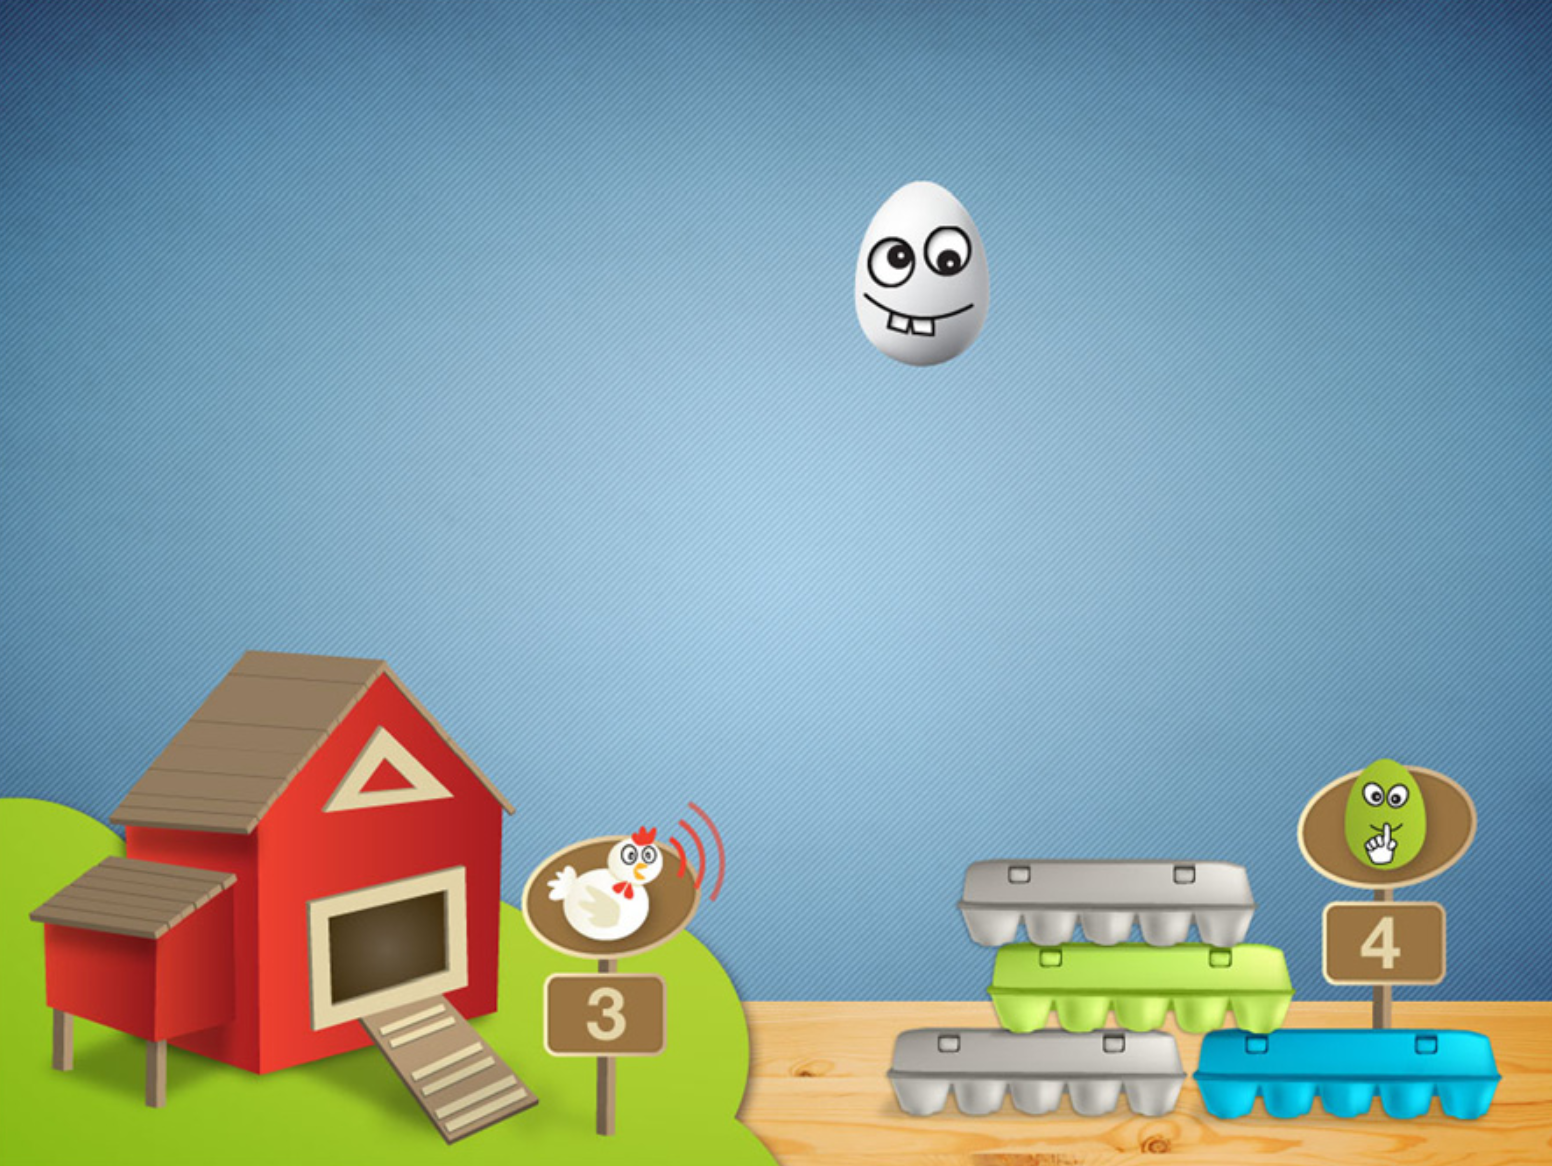
\includegraphics[width = 0.46\textwidth]{SMC2022_template_Latex/images/IpadAudiometry.png}
    \caption{Tablet audiometer gameplay screenshot \cite{ipadAudiometry}}
    \label{fig:ipadAudiometry}
\end{figure}

In a study by J. Yeung et al., a tablet-based play audiometer was implemented and evaluated to examine whether such a device can address the shortcomings (i.e., low patient cooperation) of the existing audiometry \cite{ipadAudiometry}. In the game, the child is presented with a series of objects (e.g., eggs) and is asked to categorize an object as 'silent' or 'sound-producing' by dragging the object into a container (see figure \ref{fig:ipadAudiometry}). The objects play warble tones at different frequencies. During the game, the intensity of the tones decreases until the child can no longer sort the objects correctly \cite{ipadAudiometry}. The study found that a tablet-based game is viable for testing children down to three years old. Furthermore, the study also demonstrated that there is no significant difference between the hearing threshold obtained by the device and thresholds obtained by standard play audiometry \cite{ipadAudiometry}. \newline 

The promising results from the tablet play audiometer show that it is possible to implement a computer-based game with the ability to collect the same results as traditional CPA.

\subsection{Azure Kinect for body tracking} \label{kinect}

Kinect is a popular tool used for rehabilitation and diagnostics because of the efficient skeleton tracking \cite{parkinsonKinect, balanceKinect, autismClassroom, tremorsKinect}. For children, studies show promising results when using Kinect in gamification applications \cite{autismGame, gamificationChildren}. 

\begin{figure}[h]
    \centering
    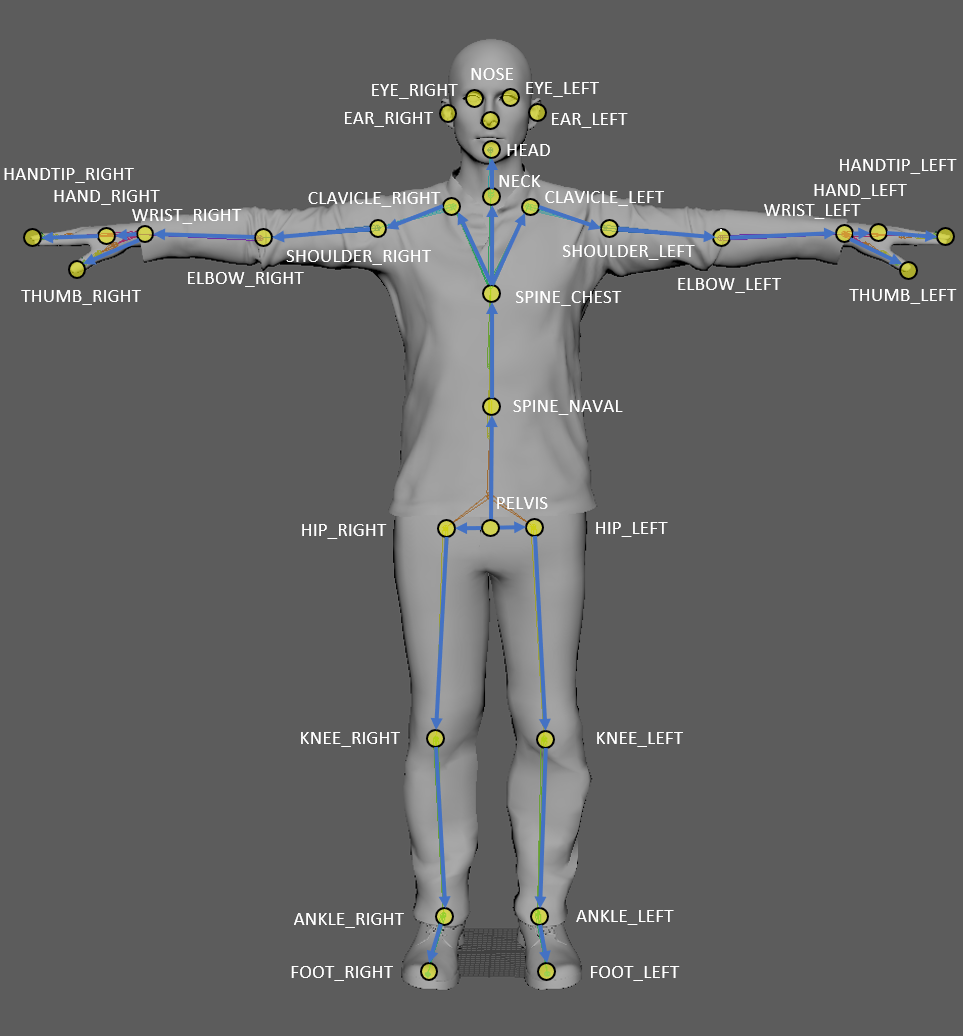
\includegraphics[width = 0.4\textwidth]{SMC2022_template_Latex/images/joint-hierarchy.png}
    \caption{The 32 tracked body joints by the Azure Kinect. All the joints are measured with position, and orientation/rotation \cite{kinectImage}.}
    \label{fig:skeletonTracked}
\end{figure}

Since 2010 three different versions of the Kinect have been released. The first version was initially designed as a game controller for the Xbox, and using an integrated RGB, and infrared camera allowed tracking users in 3D space \cite{kinectVS}. The third version of the Kinect (called Azure Kinect) has since been released in 2019 and enables skeleton tracking of 32 joints (see figure \ref{fig:skeletonTracked}) \cite{kinectVS}. A study by J. A. Albert et al., comparing the three released versions, has found that the skeleton and body tracking has been improved significantly from the first to the third version \cite{kinectVS}. \newline

The promising results from other studies and the significant body tracking development make the Azure Kinect a preferable tool for tracking the child's reaction and controlling the game. Additionally, the Azure Kinect is not body worn and hence more maneuverable and wireless, allowing the child to move more freely, creating a more immersive experience. 
\section{Implementation} \label{design}

\subsection{Test setup and system design} \label{system design}

The central part of the game is based on the same setup and methods currently operated at CHBC. An initial meeting/brainstorming with CHBC was held to map out their expectation for a digitalized and automated version of their current methods. Furthermore, a hearing test was observed to see how their current methods would translate to a 3D game. 


\begin{figure}[h]
    \centering
    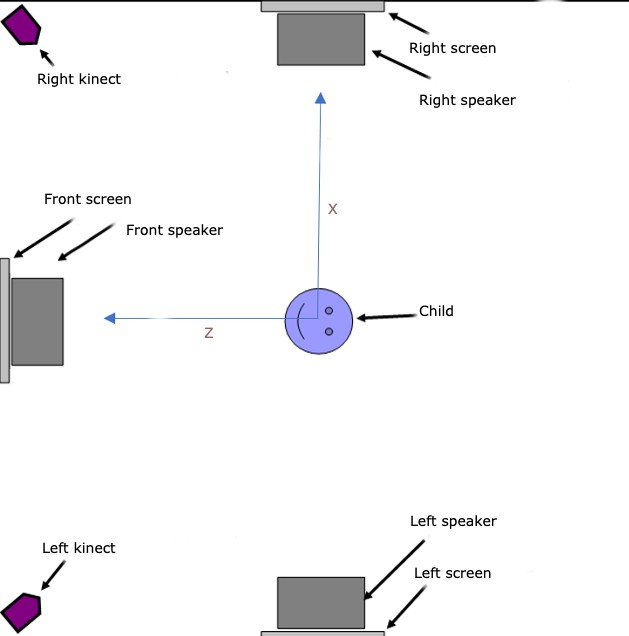
\includegraphics[width = 0.49\textwidth]{SMC2022_template_Latex/images/setup(2).jpeg}
    \caption{Testing setup for the automated CPA, based on the current setup at CHBC}
    \label{fig:setup}
\end{figure}

The first part of the design process was establishing a setup and test procedure for the new CPA, which matches the current methods and testing rooms at CHBC. The final setup can be seen in Figure \ref{fig:setup}. The child is placed in the middle of the room with a speaker and screen to the left, right, and front of the child. Two Azure Kinect in the corners are used to track the child's reaction to sound and to track gestures for controlling the game. As the game needs to be controlled precisely, also when the child is turned away from the Kinect, two Kinectsplaced at a 45$^{\circ}$ angle, should improve the skeleton tracking. The child is presented with an introduction from the front screen and speaker; afterward, the child is presented with a pure- or warble tone from either the left or right speaker. The Azure Kinect  tracks whether the child reacts correctly by looking toward the sound; if so, a fun and engaging game begins on the matching screen. The desired result is to engage the child in the test to play the game. When the game is over, the front speaker sends a message asking the child to look towards the front screen again so that a new tone can be presented.  \newline 

The design of the system was decided to be split into four different modules, which all will communicate with each other: 

\begin{enumerate}
    \item \textbf{Game-module: } This module contains all of the design (i.e., avatars and environment) and gameplay for the 3D game. This includes the design and methods for controlling the game. Furthermore, this module renders graphics on three different screens (see figure \ref{fig:setup}) . 
    \item \textbf{Kinect-module: } This module contains methods for accessing the data from the Azure Kinect to track the orientation of the child's head, the different gestures for controlling the game, and ensuring that the Kinect is following the correct body (i.e., if more than one person is in the room).
    \item \textbf{Sound-module: } This module contains methods for presenting pure- or warble tones at different frequencies and volumes (decibels) and methods for playing game sounds. This module must have access to specific outputs on the used audio interface to send sound to only the left, right or front speaker.
    \item \textbf{Control-module: } This module contains methods for changing the setup of the audio (i.e., mapping the different outputs of the audio interface) and the setup of the three different screens (i.e., what each display connected to the computer should render). Furthermore, the audiologist will use this module to control the loudness and frequency of the presented pure- or warble tones (i.e., by communicating with the Sound-module). All of this will be rendered on a separate screen, and whether the child reacted at the specific frequency and loudness will also be presented here. 
\end{enumerate}

\subsection{Game Design} \label{gameDesign}

The second part of the design process consisted of deciding on a game-play that worked well with the setup. From the initial brainstorming with CHBC, the idea of a Fruit Ninja\footnote{Fruit Ninja: https://www.halfbrick.com/games/fruit-ninja} inspired game was proposed. From the brainstorming, it was also deemed necessary that the child should be able to choose an avatar to personalize the experience. \newline

When beginning the hearing test, the child is presented with a scene in a temple with four different ninjas (see figure \ref{fig:ninjaAvatar}). 

\begin{figure}[h]
    \centering   \includegraphics[width = 0.49\textwidth]{SMC2022_template_Latex/images/avatarchoose.png}
    \caption{Gameplay screenshot from the first scene in the game. The child can choose between four different ninjas by swiping.}
    \label{fig:ninjaAvatar}
\end{figure}

The child can choose a ninja by using a swiping gesture. When the child has found the preferred ninja, the child can start the hearing test by raising their left or right hand. After a small transition, the child will now see the 3D world from the chosen Ninja's point of view and can control the ninja with body movements. Another Ninja playing the role of a \textit{distractor} gives the child an introduction to the hearing test and asks the child to be quiet and look towards the sound when presented (see Figure \ref{fig:distractor}).

\begin{figure}[h]
    \centering   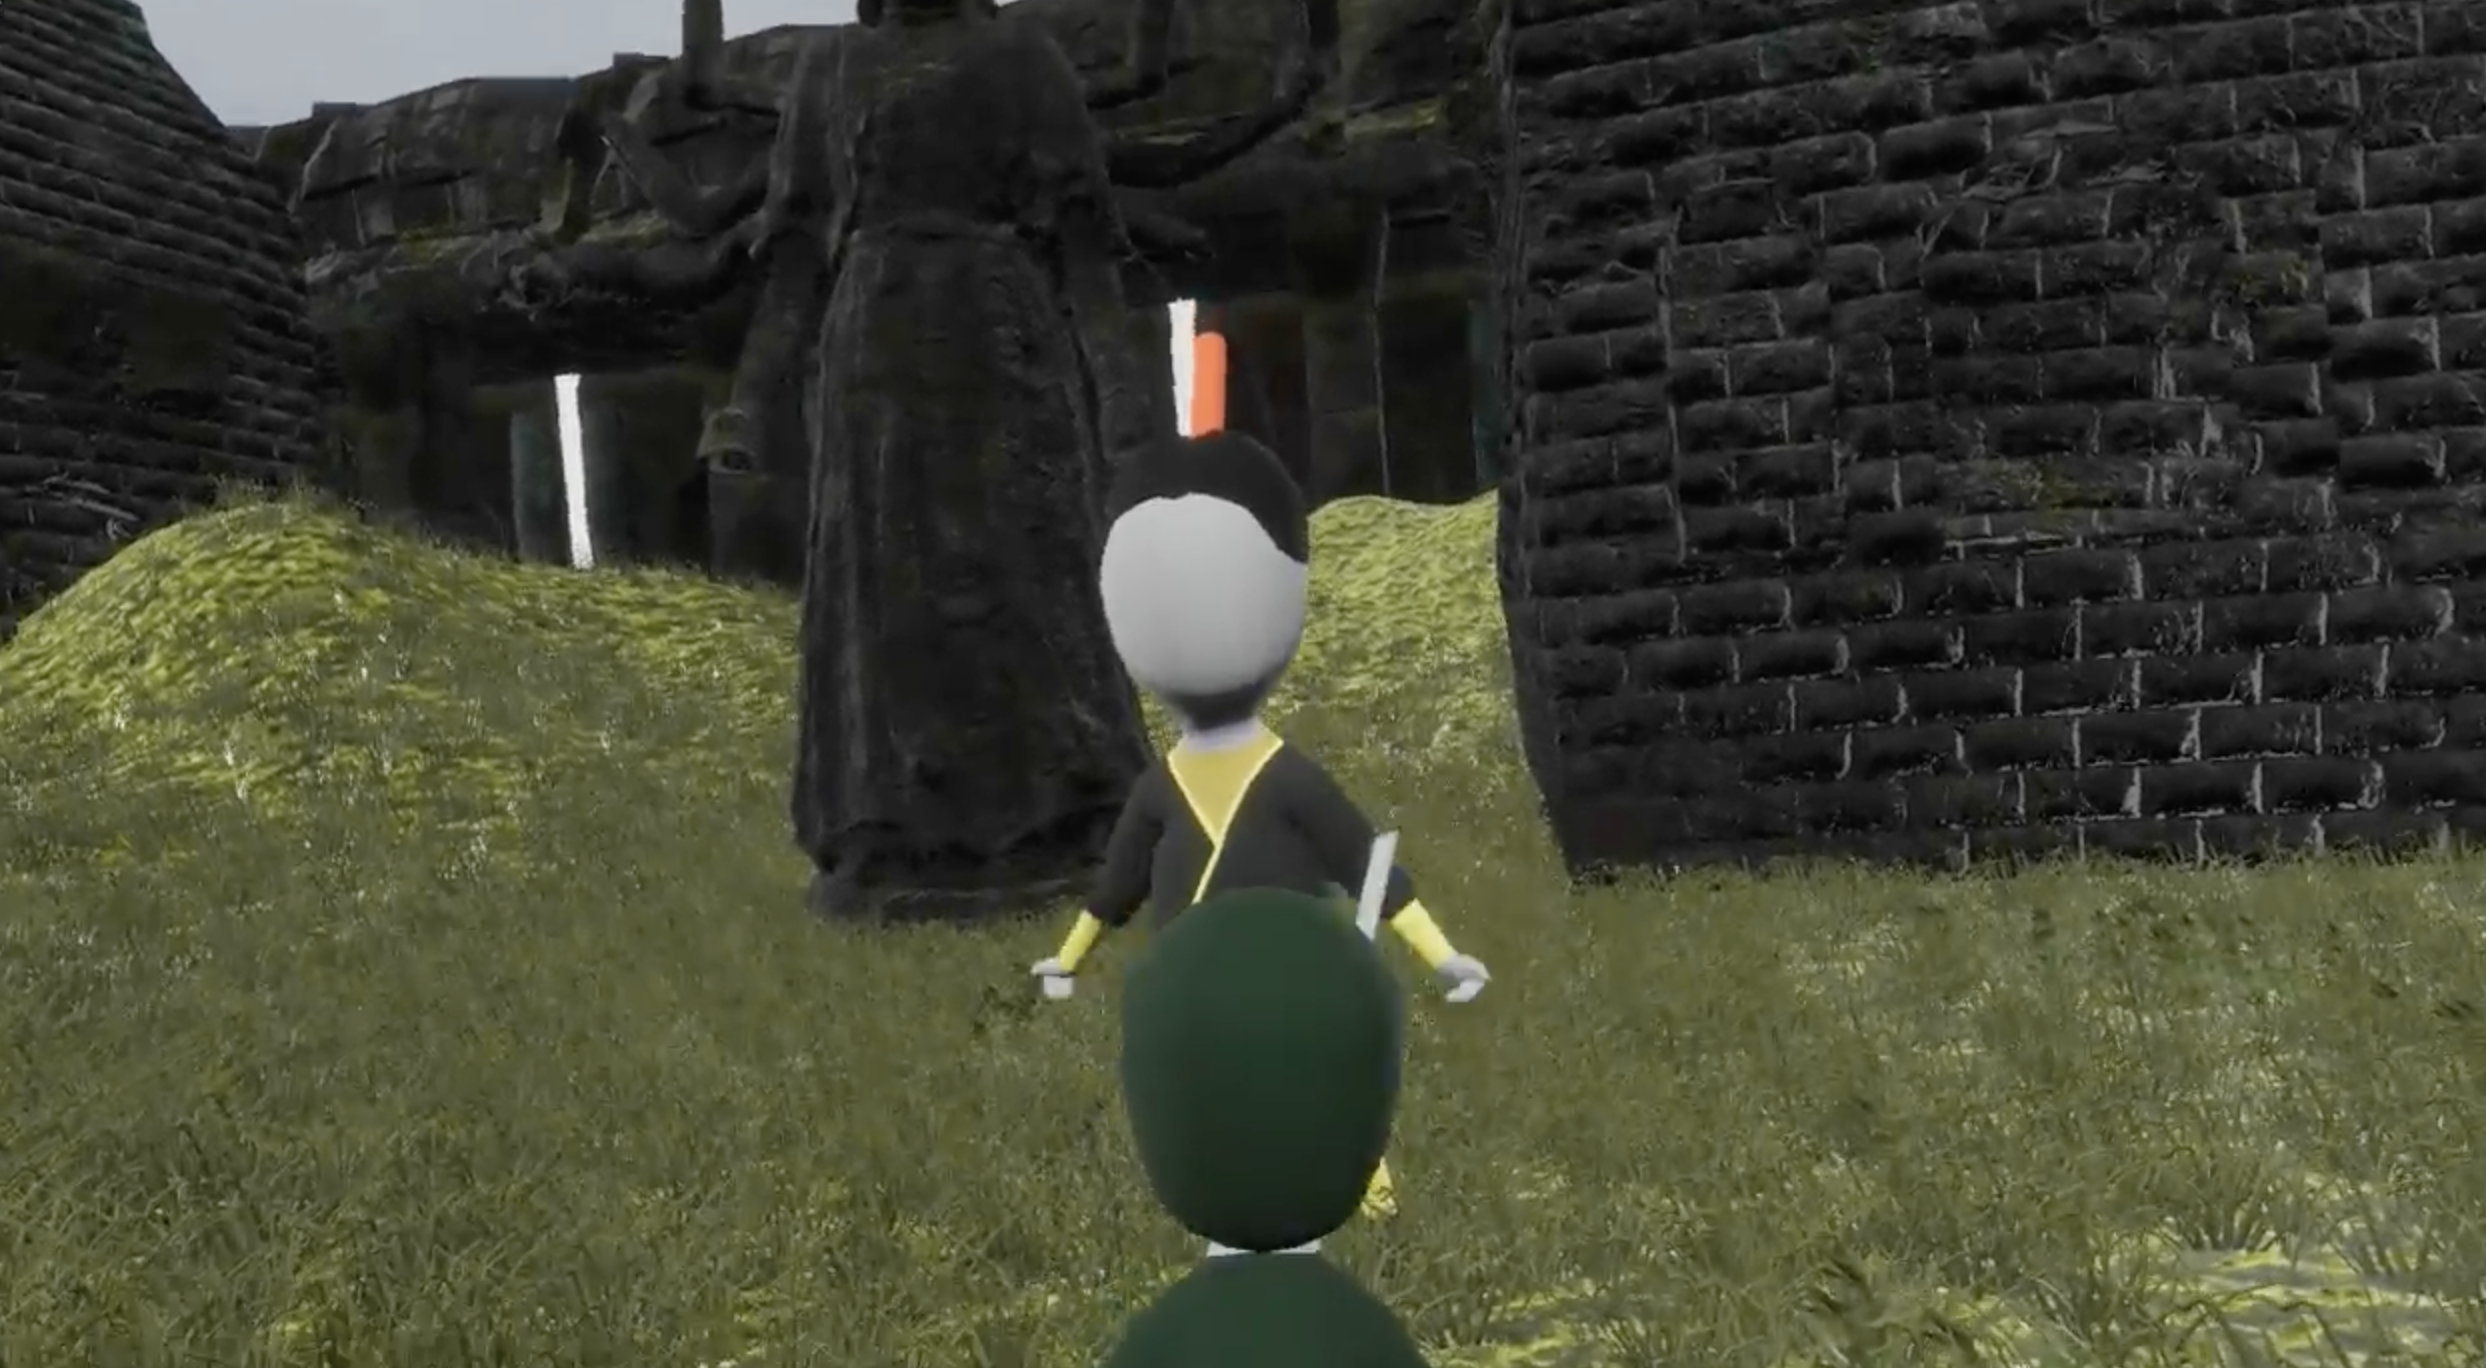
\includegraphics[width = 0.49\textwidth]{SMC2022_template_Latex/images/distractor.png}
    \caption{Gameplay screenshot from the introduction. An animated \textit{distractor} avatar introduces the child to the game.}
    \label{fig:distractor}
\end{figure}

The audiologist is now able to present a pure or warble tone, from either the left or right speaker, at a specific loudness and frequency, using the control-module (see figure \ref{fig:controlModule}). Before presenting a tone, the audiologist can choose an appropriate difficulty level for the child. The difficulty of the game ranges from 1 (easy, fruits coming slow, and are easy to hit) to 5 (hard, fruits coming fast, and are difficult to hit). 

\begin{figure}[h]
    \centering   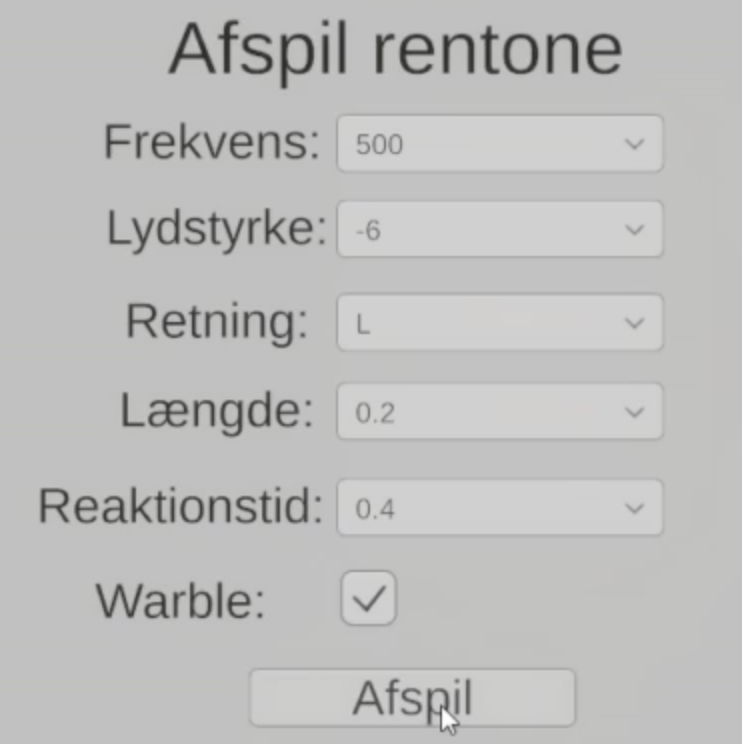
\includegraphics[width = 0.3\textwidth]{SMC2022_template_Latex/images/playtone.png}
    \caption{Screenshot from the control module. The audiologist can play a pure- or warble tone at a specific frequency and loudness.}
    \label{fig:controlModule}
\end{figure}

After choosing randomly between 3 to 5 seconds from pressing \textit{play}, the tone is presented to the child.After playing the tone, the Kinect module detects  the child's reaction; if the child reacts correctly (i.e., looking towards the sound), a short Fruit Ninja-inspired game sequence will start on the matching screen (see Figure \ref{fig:fruitNinjaGame}). When done, the \textit{distractor} asks the ninja to look towards the front screen again, and a new tone is now ready to be presented. \newline

\begin{figure}[h]
    \centering   \includegraphics[width = 0.49\textwidth]{SMC2022_template_Latex/images/ingame.png}
    \caption{Gameplay screenshot from the fruit ninja game. The child can cut fruits and gain points by slicing fruits with their movements.}
    \label{fig:fruitNinjaGame}
\end{figure}


\subsection{Technical Description} \label{technicalDescription}
The prototype was designed and implemented using the
the Unity\footnote{https://unity.com/} game-engine.

\subsubsection{Azure Kinect Implementation}
For implementation of body tracking from the Azure Kinect, the Azure Kinect Examples for Unity\footnote{https://assetstore.unity.com/packages/tools/integration/azure-kinect-examples-for-unity-149700} package was utilized. The package includes methods for body tracking and for controlling avatars. The package also includes a Unity scene, which makes it easy to calibrate two Azure Kinects, which is needed for the setup presented in Section \ref{system design}. \newline

To ensure the Azure Kinect is tracking the correct body, a maximum and minimum distance on the z and x axis was implemented (see code in appendix \ref{appendix: UserTrackingCode}). The maximum and minimum distances are changeable from the control-module. 

\label{SoundImplementation}
\subsubsection{Audiometer implementation}

For the implementation of the play audiometer, the functional programming language Faust\footnote{https://faust.grame.fr/} was used. Faust has a wrapper system, which makes it easy to export the code to a real-time DSP to be used in Unity and be initiated at a specific frequency and loudness by the sound-module. Simple sine waves in the frequency range of 0.125 kHz to 8 kHz were implemented for the pure tone implementation. For the warble tone implementation, a frequency-modulated sine wave with a modulation rate of 5 Hz and a frequency deviation of 10\% was implemented (see section \ref{WarbleTones}). The modulation index is calculated as a ratio between the frequency deviation (in Hz) and the modulation rate (in Hz). This results in the following equation for the warble tone: 

\begin{equation}
    wt(f_{c},f_{m},f_{d}) = sin(2\pi f_{c}t+\frac{f_{c}f_{d}}{f_{m}}sin(2\pi f_{m}t)),
\end{equation}
\begin{footnotesize}
\textit{where $f_{c}$ is the center frequency in Hz, $f_{m}$ is the modulation rate in Hz and $f_{d}$ is the frequency deviation in percentages (e.g. 5\% frequency deviation is $f_{d} = 0.05$). }
\end{footnotesize} \newline


As the warble tone is generated in real-time by the Faust DSP in Unity, the frequency deviation and modulation rate is implemented to be changeable within the game controls in the control-module. As mentioned in section \ref{WarbleTones}, this give the possibility for the warble tone in the prototype to match any audiometer. The implementation in Faust code can be found in appendix \ref{appendix:faustCode}.


\subsubsection{Audio setup}

For the sound to work with the setup presented in section \ref{system design}, the sound-module must have access to specific outputs on a specific audio interface. As this functionality is not natively supported in Unity, the AudioStream\footnote{https://assetstore.unity.com/packages/tools/audio/audiostream-pcm-audio-for-unity-65411} package was utilized. The package includes methods for accessing all audio interfaces connected to the computer and channeling audio to specific audio outputs. All this is implemented to be controlled from the control-module to make the setup easy for any interface (see Figure \ref{fig:audioInterface}). 

\begin{figure}[h]
    \centering   
    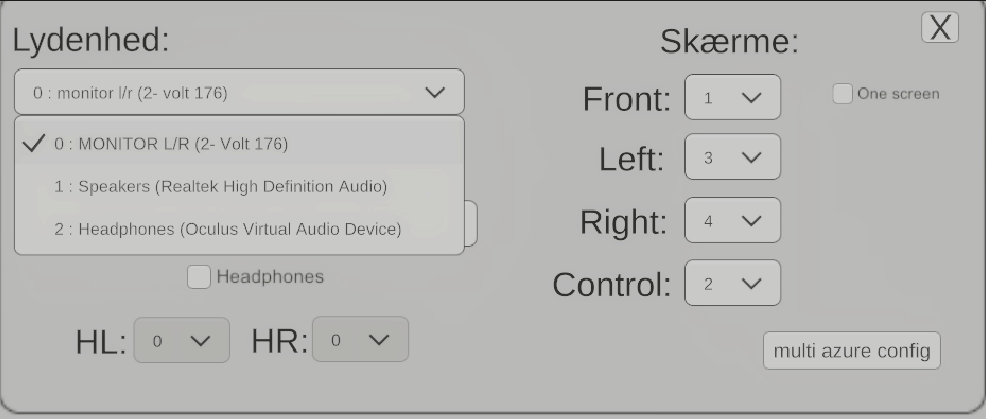
\includegraphics[width = 0.49\textwidth]{SMC2022_template_Latex/images/14.12.2022_12.41.16_REC.png}
    \caption{Screenshot from the control-module. Utilizing AudioStream, it is possible to change the targeted audio interface and which output on the interface is the front, left, and right speaker.}
    \label{fig:audioInterface}
\end{figure}



\section{Evaluation}

\subsection{Methods}
For the initial evaluation, the prototype was presented to audiologists at CHBC on two different occasions. The audiologist's opinions were gathered using the think-aloud method \cite{thinkAloud} and non-participatory observation methods during gameplay, along with the possibility of asking questions afterward. The main goal of the evaluation was to gather feedback on the prototype's functionality, whether the audiologist understood the concept, and whether the audiologist thought a child would be able to understand the game. As it is the audiologists who conduct hearing tests every day, it is essential that they believe the concept and gameplay are ready before testing on the target group. As of writing this report, it has not been possible to set up the final test as presented in section \ref{system design}. Instead, a simpler setup was used with only one Kinect, and one screen rendering all gameplay. Because of the limited time frame of this project, the prototype has yet to be tested on children. 

\subsection{Results} \label{results}

The following observations and results were gathered from the tests:
\begin{itemize}
    \item Several audiologists found it challenging to control the ninja in the way they wanted. For example, when slicing fruits, their movements were fast, which the Azure Kinects had difficulty tracking. 
    \item One audiologist seemed confused about which part of the game was the actual hearing test. The question \textit{"Are the fruits not supposed to play tones?"} was asked, pointing to the audiologist not fully understanding the test. 
    \item One audiologist pointed out that all screens should fade to black when a tone is presented. The audiologist mentioned this, as the visuals might distract the child from listening to the sound. Furthermore, it was said that only the screen with active gameplay should render any graphics. 
    \item Several audiologists mentioned the Fruit Ninja game to be too long. Instead, they said the game should be short, with time only to slice a couple of fruits. 
    \item Generally, the audiologist found the gameplay engaging and was, for the most part, able to understand the concept. However, one audiologist raised concerns about the younger children (i.e., 3-year-olds), who may not understand the game entirely.
\end{itemize}

\subsection{Discussion} \label{disussion}

% Is the game ready for children?? 
Based on the results from the preliminary evaluation (see section \ref{results}), the audiologist generally found the concept appealing. However, some issues with the prototype were pointed out, showing that it still needs further implementation before it is ready to test on the target group. As mentioned, it was observed that one audiologist had a hard time fully understanding which part of the game was the actual hearing test. Furthermore, one audiologist pointed out that the Fruit Ninja gameplay was too long. This feedback points to the hearing test part of the game needing to be more integrated with the Fruit Ninja gameplay. The long pauses in the hearing test might distract the child from the test itself and prolong it too much. It is crucial that further testing assess whether this is the case, and if so, the gameplay might need to be limited and integrated more.   \newline

As one audiologist mentioned, the graphics must not distract the child when presenting tones. Removing the graphics when presenting tones and only having graphics rendered on one screen at a time is easily implementable and should help. Generally, this raises the concern of whether a 3D game and its visuals will end up distracting more than it engages. This will have to be assessed further to see whether the visual needs to be removed, so the graphics is less distracting. Another concern is whether the gameplay is too advanced, especially for younger children. Slicing fruits should be an easy task; however, if the child does not understand how to control the avatar, this might cause some issues. \newline

It was observed that the audiologist had difficulty controlling the avatar in the way they wanted. The precision and small delay when tracking bodies using the Azure Kinect might cause a problem when children play. If the child cannot play the game correctly because of precision and delay issues, this might cause the child to become frustrated with the game and, thereby, the hearing test. However, precision issues might be solved when testing using the exact setup presented in section \ref{system design}. It should be tested whether the complete test setup solves these issues; if not, the way the avatar is controlled might need to be changed. \newline 



\input{SMC2022_template_Latex/discussion.tex}
\section{Conclusion} \label{Conclusion}
A test setup has been developed based on the current methods used at CHBC, a system design was created, and a Fruit Ninja-Inspired play audiometer was designed and implemented to be controlled by the Azure Kinect. The audiologist generally found the new methods appealing and could see the potential; however, several issues were pointed out, such as distracting graphics when presenting tones and gameplay being too long. This indicates the prototype needs further implementation before testing on the target group. Solving these issues should help avoid problems in further iterations. Nevertheless, when testing on children, it is essential to assess whether (1) the visuals are too distracting and need to be toned down, (2) the gameplay distracts the child from the hearing test, and (3) whether delay and tracking issues with the Azure Kinect can be kept to a minimum when tracking the children. 
\input{SMC2022_template_Latex/Acknowledgement.tex}
\newpage
\bibliography{smc2022bib}

\newpage
\onecolumn
\begin{appendices}
\section{Kinect: User tracking code} \label{appendix: UserTrackingCode}
\begin{lstlisting}[linewidth=\columnwidth,breaklines=true]
IEnumerator DetectPlayer()
{
    while (trackingOn)
    {
        if (KinectManager.Instance.IsInitialized())
        {
            users = KinectManager.Instance.userManager.alUserIds;

            tempPlayerDetected = false; 

            foreach(ulong user in users)
            {
                if (KinectManager.Instance.IsUserTracked(user))
                {

                    Vector3 userPos = KinectManager.Instance.GetJointPosition(user, KinectInterop.JointType.Head);

                    if(userPos.x > xMin && userPos.x < xMax && userPos.z > zMin && userPos.z < zMax)
                    {

                        if(detectedUserID != user)
                        {
                            detectedUserID = user;
                        }

                        tempPlayerDetected = true;
                        break;
                    }
                }
            }

            if(tempPlayerDetected == true)
            {
                StartGestureTracking(gesturesToTrack, detectedUserID);
                playerDetected = true;
            }
            else
            {
                StopGestureTracking(gesturesToTrack, detectedUserID);
                playerDetected = false;
            }
        }

        yield return new WaitForSeconds(DetectTime);
    }
}
\end{lstlisting}

\newpage
\section{Audiometer: Faust Code} \label{appendix:faustCode}
\begin{lstlisting}[linewidth=\columnwidth,breaklines=true]
import("stdfaust.lib");

audiometer = wt
with {
    // all variables
    // center frequency
    fc = nentry("Center frequency",125,125,8000,125);
    // modulation rate
    fm = nentry("Modulation rate",5,0,32,0.01); 
    // frequency deviation
    fd = nentry("Frequency deviation",0.05,0,0.1,0.001);
    // pure or warble tone
    pOrW = nentry("Pure tone or warble tone", 0,0,1,1); 
    // modulation index
    mi = (fc*fd)/fm; 
    
    // equation
    wt = os.osc(fc + (1 == pOrW) * (mi * os.osc(fm)));
};

trigger  = nentry("ON/OFF", 1,0,1,1): si.smoo;
process = audiometer * trigger <: _,_;
\end{lstlisting}
\end{appendices}




\end{document}
